\documentclass[handout]{beamer}
\usepackage[frenchb]{babel}
\usepackage[T1]{fontenc}
\usepackage[utf8]{inputenc}
\usepackage{graphicx}
\usepackage{subfig}

% functions to plot
\def\func(#1){(#1)*(1-(#1))}
\hypersetup{colorlinks = true,linkcolor = blue,urlcolor  = blue}
            
\newcommand{\qGraph}[1]{\begin{center} \includegraphics[width =
\textwidth]{#1}\end{center}}

\newcommand{\mcl}{\mathcal}

\addtobeamertemplate{navigation symbols}{}{%
    \usebeamerfont{footline}%
    \usebeamercolor[fg]{footline}%
    \hspace{1em}%
    \insertframenumber/\inserttotalframenumber
}

\newenvironment{iPar}[1]{\textbf{#1} \begin{itemize}}{\end{itemize}}

\newcommand{\inc}{{inc}}
\newcommand{\cp}{{cmp}}
\newcommand{\bull}{$\bullet\;$} 

\newcommand{\esp}{\mathbf{E}} \newcommand{\ul}[1]{\underline{#1}}
\newcommand{\ol}[1]{\overline{#1}} \newcommand{\ora}[1]{\textbf{#1}}
\newcommand{\wh}{\widehat}
\newcommand{\mdp}{\medskip \pause}
\newcommand{\mc}{\mathcal}

\title{Intertemporal Choice}
\author{Microeconomics \\ 20851}
\date{}

\begin{document}

\frame{\titlepage}

\section[Outline]{}
\frame{\tableofcontents}

\section{}


\begin{frame}\frametitle{Itinéraire}

\begin{iPar}{Jusqu'à maintenant}
\item Choix du consommateur
\item Effets prix et richesse
\item Risque 
\end{iPar}\mdp

\begin{iPar}{Ce cours: temps}
\item Pour comprendre l'épargne, l'achat de bien durable
\end{iPar}\mdp

\begin{iPar}{Plus tard}
\item  Le bien-être
\item  Équilibre de marché en situation d'échange
\item  La production des firmes
\item Le comportement stratégique des firmes
\item Les enchères
\end{iPar}

\end{frame}

\section{Préférences}

\begin{frame}\frametitle{Préférences}

Les gens ont en général une préférence pour le présent (si bénéfice) et pour retarder dans le futur (si coût):

\begin{itemize}
\item Un café maintenant vs. à la pause?
\item Aller au gym aujourd'hui vs. demain?
\item Épargner aujourd'hui pour consommer à la retraite?
\end{itemize}

\end{frame}


\begin{frame}\frametitle{Utilité escomptée}

Si $u(C_t)$ est l'utilité de la consommation au moment $t$, l'utilité escompté pour un plan de consommation $\textbf{C} = (C_1,...,C_T)$ est :


$$ DU(\mathbf{C}) = \sum_{t=1}^T \delta^{t-1} u(C_t) $$

$\delta$ $\in [0,1]$ est le facteur d'escompte (patience) alors que $\mathbf{C} = (C_1,...,C_T)$. La relation entre le taux d'escompte, $\rho$ et le facteur $\delta$ est donnée par: 

$$ \delta = \frac{1}{1+\rho} $$

\end{frame}

\begin{frame}\frametitle{Taux marginal de substitution (TMS)}

Si $T=2$, alors $$ DU(\textbf{C}) = u(C_1) +  \delta u(C_2) $$. La différentielle totale donne le TMS: 

$$ \frac{\partial C_2}{\partial C_1}\rvert_{dDU=0} = -\frac{u'(C_1)}{\delta u'(C_2)}$$

Les préférences intertemporelles sont caractérisées par: 

\begin{itemize}
\item Le facteur d'escompte ($\delta$)
\item La forme de $u$. 
\end{itemize}

\textbf{Exercice A}: Trouvez le TMS pour $u(C_t) = \log c_t$

\end{frame}


\begin{frame}{Comment estimer les taux d'escompte?}

Expérience au Danemark  (Harrison, Lau et Williams, 2002)

\begin{figure}
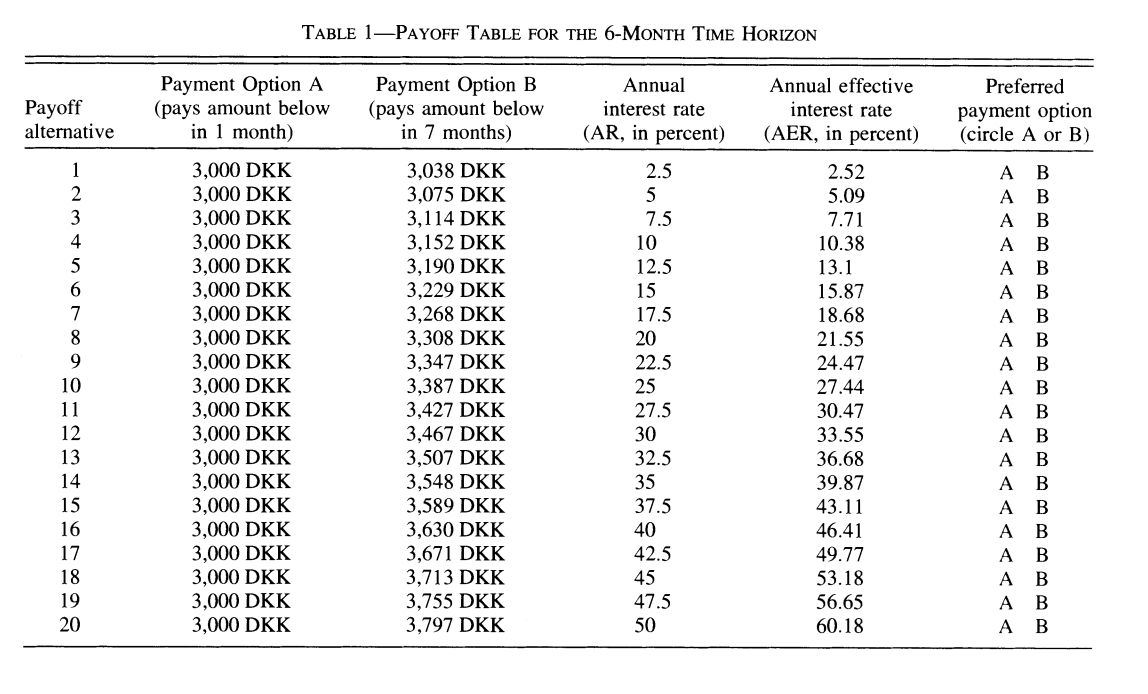
\includegraphics[scale=0.5]{MPL.png}
\end{figure}


\end{frame}

\begin{frame}{Résultats taux d'escompte}

Expérience au Danemark  (Harrison, Lau et Williams, 2002)

\begin{figure}
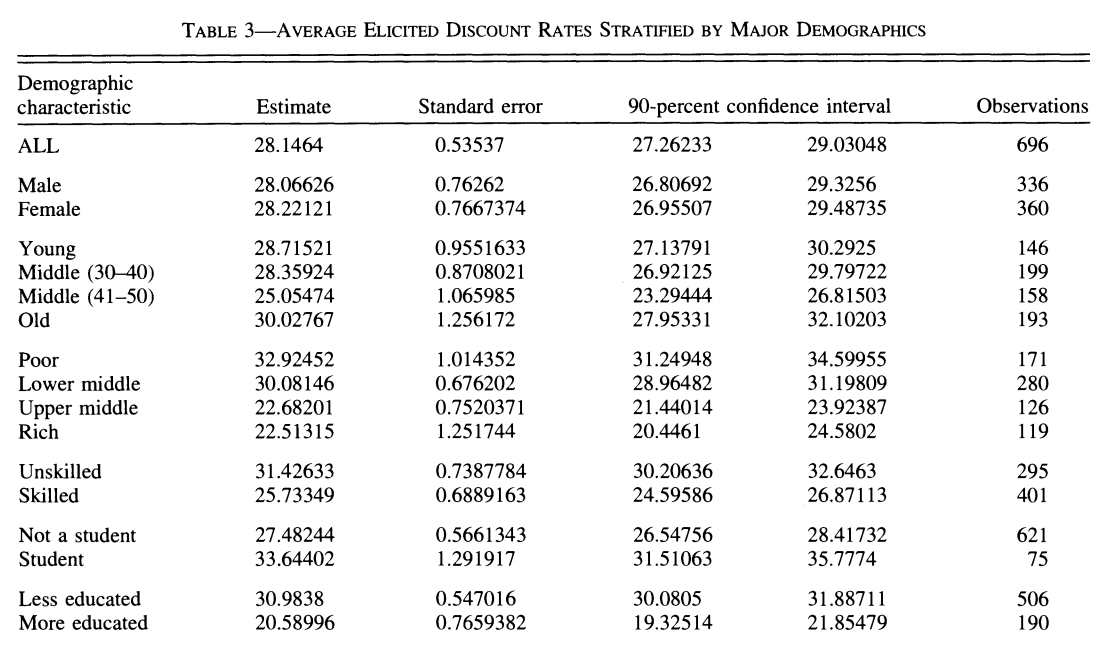
\includegraphics[scale=0.5]{Results.png}
\end{figure}

\end{frame}

\section{Contrainte Intertemporelle}

\begin{frame}{Intérêt et Marchés financiers}

Les institutions financières nous offre $r_S$ pour chaque dollar déposé (épargné). Elles demandent une compensation $r_D$ pour chaque dollar prêté

Pour le moment supposons $r_D = r_S = r$. 

\end{frame}

\begin{frame}{Ressources}

Les ressources proviennent de deux sources:
\begin{itemize}
\item la richesse initiale: $W_0$. 
\item les revenus dans les deux périodes, $Y_1$, $Y_2$. 
\end{itemize}

La valeur présente des ressources est : 

$$ VP_W = W_0 + Y_1 + \frac{Y_2}{1+r} $$
 
\end{frame}

\begin{frame}{Contrainte}

La valeur présente des consommations des deux périodes est: 

$$VP_C = C_1 + \frac{C_2}{1+r}$$. 

Ainsi la contrainte intertemporelle est $ VP_C \leq VP_W $:

$$ C_1 + \frac{C_2}{1+r} \leq W_0 + Y_1 + \frac{Y_2}{1+r}  $$

\end{frame}

\begin{frame}{Emprunt et Épargne}

On peut écrire la contrainte tel que :

$$ (1+r)(W_0 + Y_1 - C_1) \ge  C_2 - Y_2 $$

Donc,

\begin{itemize}
\item L'individu qui épargne dans la première période (côté gauche positif) peut consommer plus que son revenu dans la deuxième (côté droit positif).
\item L'individu qui emprunte dans la première période (côté gauche négatif) doit consommer moins que son revenu dans la deuxième (côté droit négatif).
\end{itemize}

\end{frame}


\begin{frame}{Visuel}

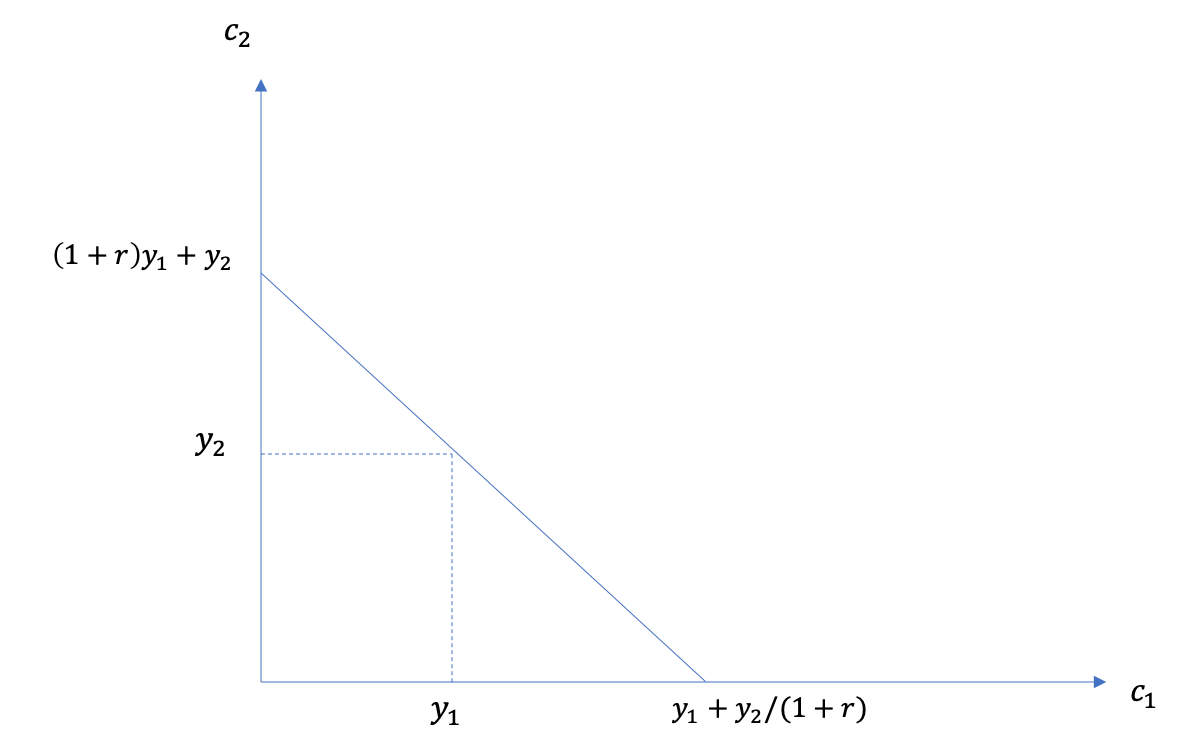
\includegraphics[scale=0.5]{budget.png}

\end{frame}


\begin{frame}{Exemple: Système contributif de retraite}

Un régime à prestation déterminée forçe l'épargne dans la première période. 
\begin{itemize}

\item Le revenu en deuxième période est $Y_2 = \phi Y_1$ avec $\phi \in [0,1]$. 
\item Le revenu de première période est amputé d'une contribution, $\tau Y_1$. 

\end{itemize}

La contrainte de ressources est donc: 

$$ C_1 + \frac{C_2}{1+r} \leq W_0 + (1-\tau)Y_1 + \frac{\phi Y_1}{1+r}  $$

Le taux de contribution $\tau$ est choisi par des actuaires tel que : 

$$ \tau Y_1 = \frac{\phi Y_1}{1+r_P} \to \tau = \frac{\phi}{1+r_P} $$

où $r_P$ est le taux de rendement du régime. Si $r_P = r$, la contrainte budgétaire ne change pas! Les consommations ne changement pas quand $\phi$ augmente et donc l'épargne s'ajuste (effet d'éviction).

\end{frame}

\begin{frame}{Différentiel de taux}

\textbf{Exercice B}: À quoi ressemble la contrainte si $r_S<r_D$?

\textbf{Exercice C}: Comment exprimer une situation où l'individu ne peut emprunter?

\end{frame}

\section{Choix optimal}

\begin{frame}{Maximisation}

Le problème est (posons $W_0=0$ pour simplifier):

$$ \max_{C_1,C_2} \{ u(C_1) + \delta u(C_2) : C_1+C_2/(1+r) \leq Y_1 + Y_2/(1+r)\}  $$

Deux approches: 
\begin{enumerate}
\item Approche directe (substitution contrainte)
\item Lagrangien	
\end{enumerate}


\end{frame}

\begin{frame}{Condition optimalité}

Le lagrangien donne les 3 CPO:

\begin{eqnarray}
 u'(C_1) - \lambda = 0  \\
\delta u'(C_2) - \lambda /(1+r) = 0  \\
C_1+C_2/(1+r) - Y_1 - Y_2/(1+r) = 0  
\end{eqnarray}

De (1) et (2) on déduit que : 

$$ \frac{u'(C_1)}{\delta u'(C_2)} = 1+r $$

En ré-arrangeant et dénotant $R=1+r$, on a l'équation d'Euler: 
$$ u'(C_1) = R\delta u'(C_2) $$
\end{frame}

\begin{frame}{Visuel}
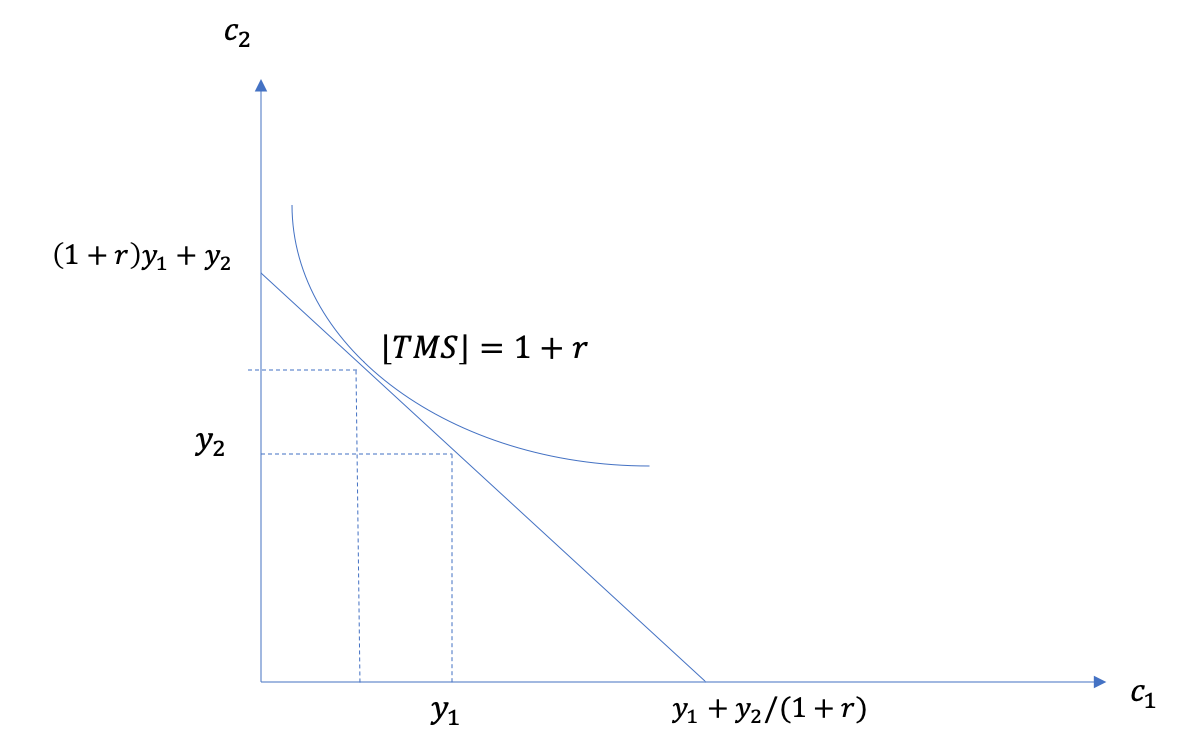
\includegraphics[scale=0.5]{optimal.png}
\end{frame}

\begin{frame}{Exemple}

\textbf{Exercice D}: Résoudre pour le choix optimal de $C_1$ et $C_2$ si $u(C)=\frac{C^{1-\sigma}}{1-\sigma}$

\end{frame}

\begin{frame}{Exemple: Épargne-t-on assez?}

Une large littérature et un important débat public à savoir si les gens épargnent assez pour la retraite.

\begin{figure}
	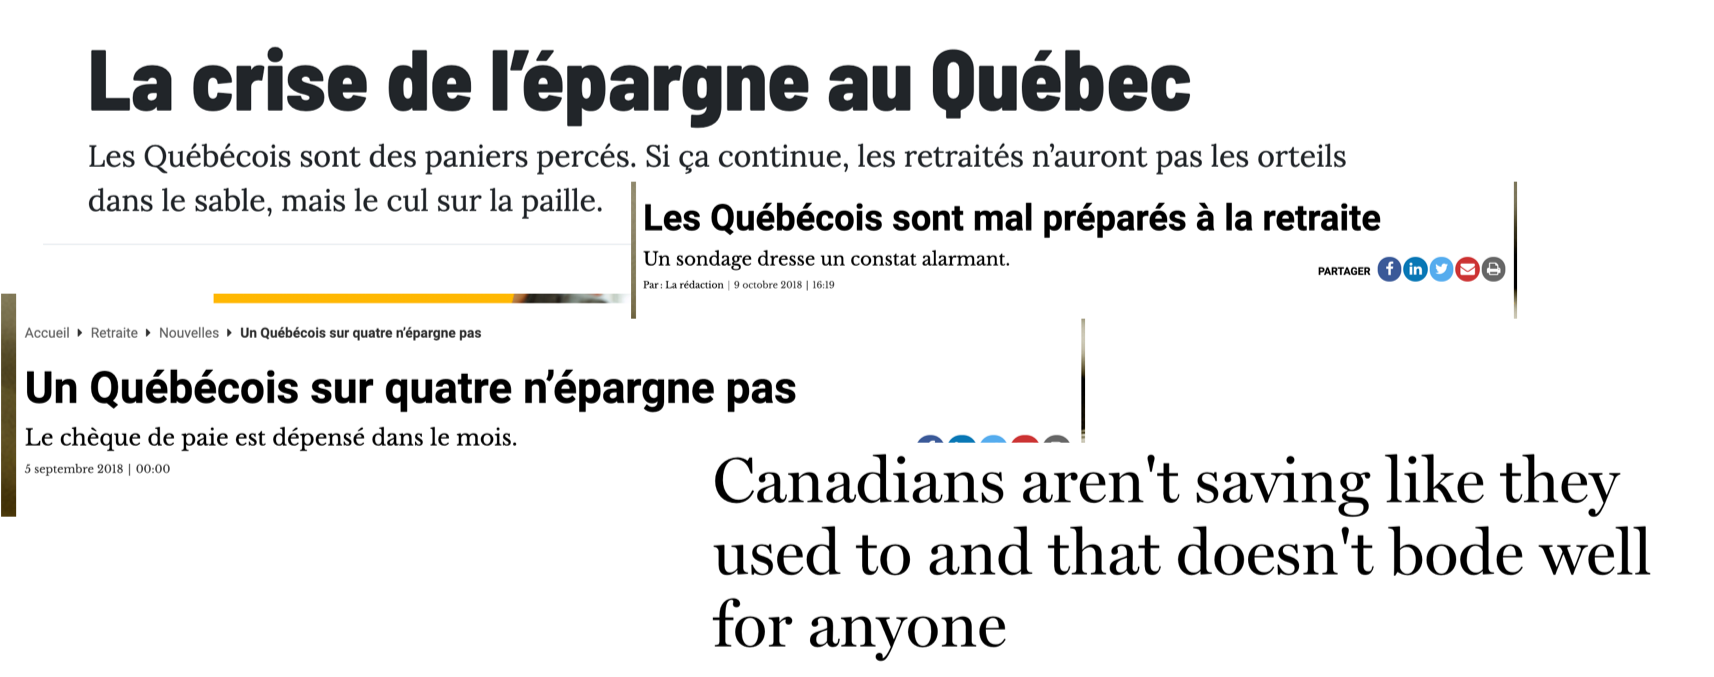
\includegraphics[scale=0.4]{retraite.png} 
	\caption{Le Conseiller, Globe and Mail, L'Actualité}
\end{figure}

\end{frame}

\begin{frame}{Le taux de remplacement}

\begin{figure}
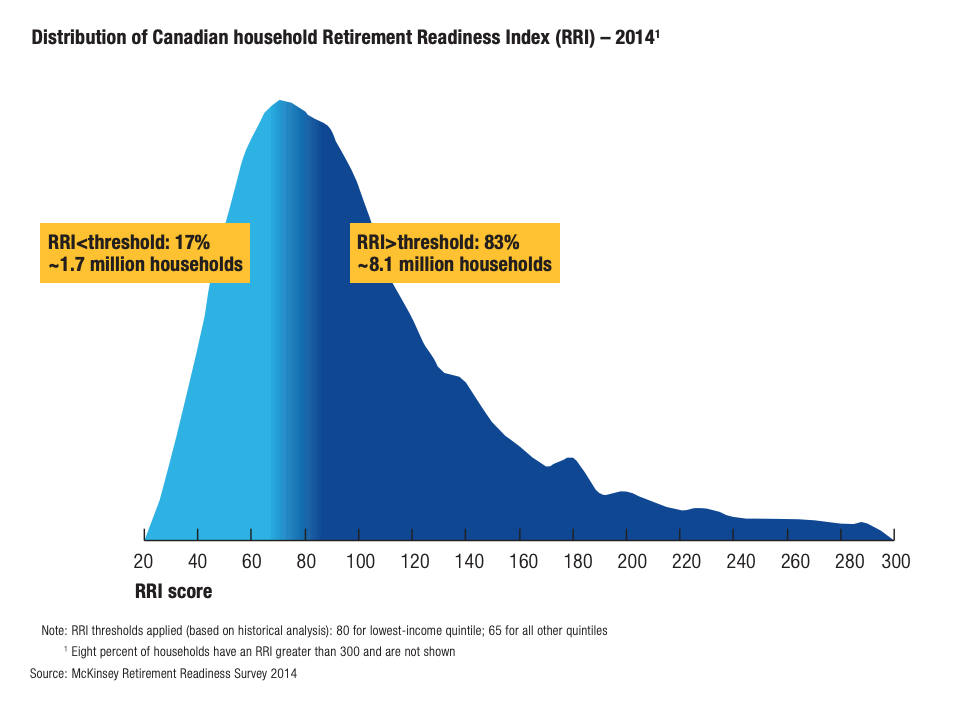
\includegraphics[scale=0.4]{mckinsey.png} 
\caption{McKinsey (2015)}
\end{figure}
	
\end{frame}

\begin{frame}{Niveau optimal d'épargne}

Que nous dit la théorie sur combien les gens devraient épargner?\vspace{0.25in}

\textbf{Exercice E}: Trouvez l'expression de l'épargne accumulée optimale au début de la période 2 si $u(C)=\frac{C^{1-\sigma}}{1-\sigma}$ et la contrainte est donnée par:

$$ C_1 + \frac{C_2}{1+r} \leq (1-\tau)Y_1 + \frac{\phi Y_1}{1+r}  $$ 

\end{frame}


\begin{frame}{Exemple: Épargne-t-on assez?}

On peut prendre en compte les préférences en simulant combien les gens doivent épargner (et comparer).

\begin{figure}
	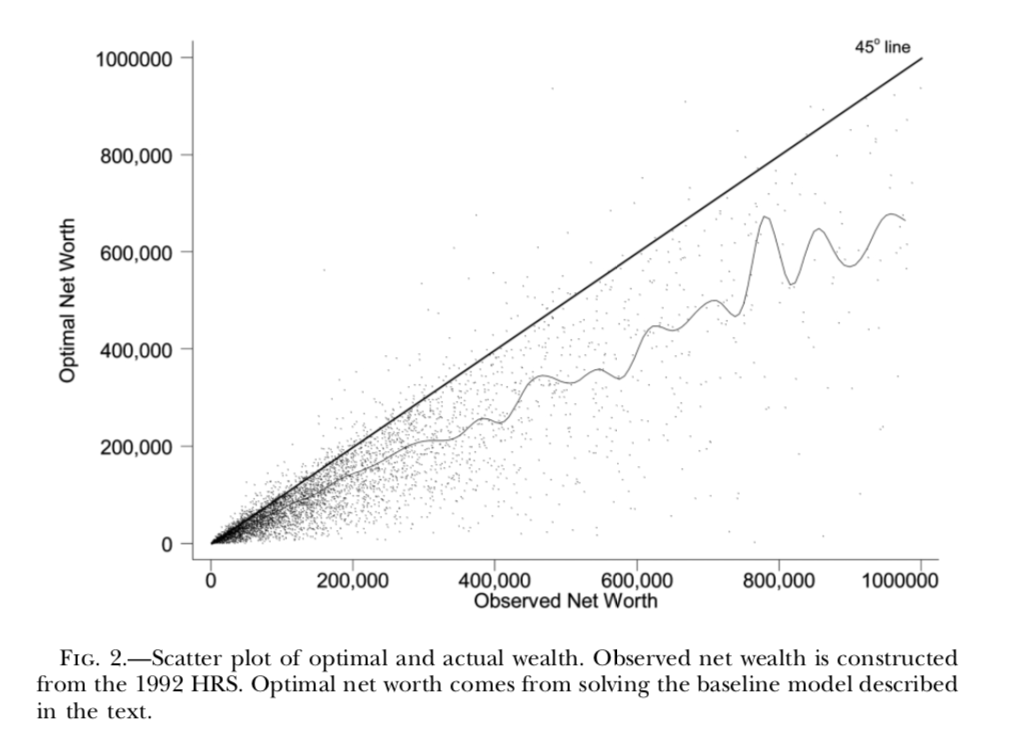
\includegraphics[scale=0.4]{savings.png}
	\caption{Scholz et al. (2007, Journal of Political Economy)}
\end{figure}


\end{frame}

\section{Biais pour le présent}

\begin{frame}{Exemple: Choix d'un film}

Vous devez choisir le film à regarder ce soir et celui que vous regarderez la semaine prochaine: 

\begin{figure}
\subfloat[Mommy (Xavier Dolan)]{
\includegraphics[scale=0.5]{Mommy.png}}
\subfloat[Les Boys (Louis Saia)]{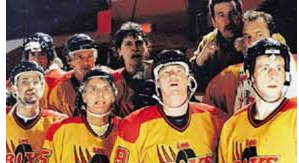
\includegraphics[scale=0.5]{boys.png}}

\end{figure}

\end{frame}

\begin{frame}{Préférences biais-présent}

Supposons que Mommy a un bénéfice immédiat de 4 et un bénéfice futur de 4 mais que Les Boys a un bénéfice immédiat de 7 (aucun bénéfice futur). \vspace{0.25in}

\textbf{Exercice E}: Quelle est l'utilité escompté si décision aujourd'hui et que $\delta=1$. Si décision la semaine prochaine?

\end{frame}


\begin{frame}{Préférences biais-présent}

Laibson (1997) propose l'utilité escompté quasi-hyperbolique: 

$$QH(\mathbf{c}) = u(C_1) + \beta \sum_{t=2}^T \delta^{t-1} u(C_t)$$

\textbf{Exercice F}: Quel est le TMS entre les consommations $C_1$ et $C_2$? Et $C_2$ vs. $C_3$? Comparer avec espérance d'utilité.

\end{frame}

\begin{frame}{Préférences biais-présent}

Dans le cas des deux films, supposons $\beta=0.5$. 
\vspace{0.5in}

\textbf{Exercice G}: Quel film est choisi si choix aujourd'hui avec des préférences biaisées pour le présent? Si choix la semaine prochaine?

\end{frame}

\begin{frame}{Exemple: Pourquoi acheter l'abonnement au Gym?}

Une passe pour une visite coûte 10\$. Le coût par visite de ceux achetant un abonnement dépasse largement 10\$. 

\begin{figure}
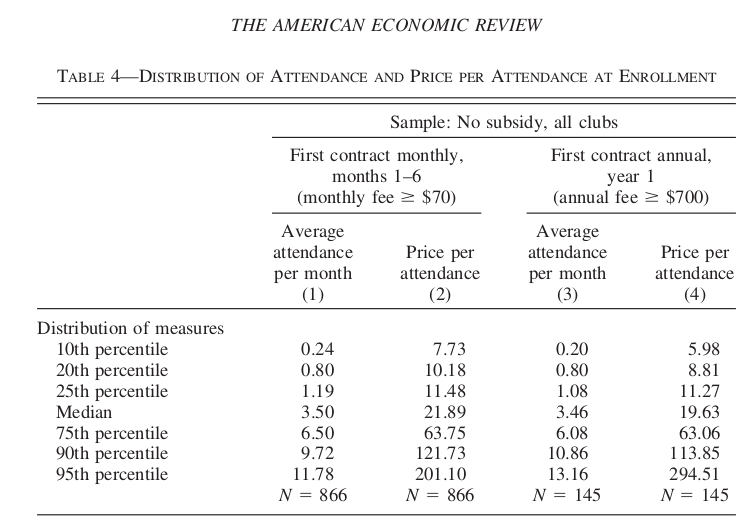
\includegraphics[scale=0.3]{Gym.png}
\caption{Della Vigna et Malmendier (2006)}
\end{figure}

\end{frame}

\begin{frame}{Exemple: Comment aider les gens à épargner?}

\begin{itemize}
\item Commencer à épargner est similaire à l'exercice: coûteux à court terme, bénéfices à long-terme.
\item On pourrait décider de changer l'option par défaut (mécanisme bien connue en psychologie): opt-in vs. opt-out (nudges, relié à la théorie des perspectives)
\item Shea et Madrian (2001, QJE) montre qu'à court terme l'épargne augmente beaucoup dans les firmes qui utilisent le opt-out
\end{itemize}

\end{frame}

\begin{frame}{La puissance des nudges}
La participation augmente de manière marquée chez les nouveaux employés.
	\begin{figure}
		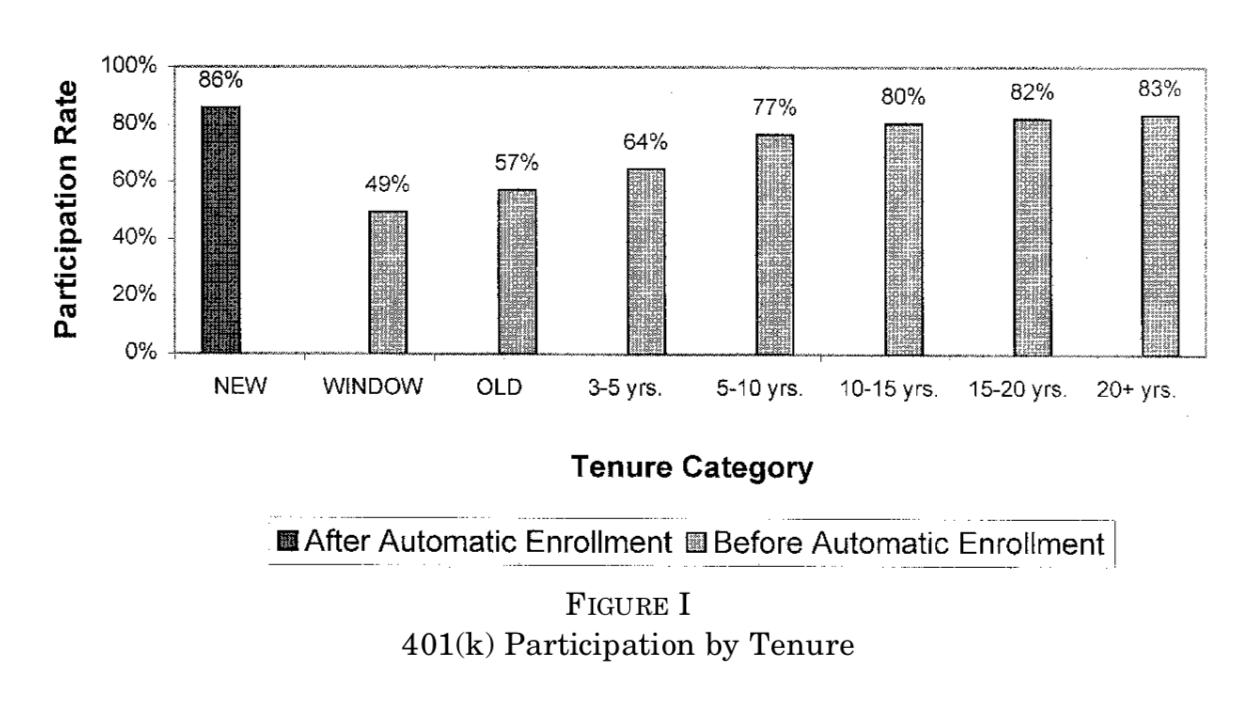
\includegraphics[scale=0.45]{shea.png}
		\caption{Shea et Madrian (2001, QJE)}
	\end{figure}
\end{frame}


\end{document}




